%chktex-file 44

% \subsection{Ιστορία και Περιγραφή Συσκευής}\label{subsec:hololenseDescription}
Το 2015, η Microsoft παρουσίασε τα γυαλιά μικτής πραγματικότητας Microsoft Hololens, όντας το πρώτο `ασύρματο' ολογραφικό υπολογιστικό σύστημα, δηλαδή δεν ήταν απαραίτητη η χρήση καλωδιών για τη λειτουργία του, καθιστώντας το πλήρως φορητό~\cite{a2021_hololens}. Η πρώτη έκδοση του headset, Development Edition, έγινε διαθέσιμη το 2016. Η συσκεύη αυτή, καθώς και οι εκδόσεις που ακολούθησαν, ενσωματώνουν την πλατφόρμα Windows Mixed Reality, η οποία βασίζεται στο λειτουργικό σύστημα Windows 10~\cite{kipman_2016_announcing}. Η συσκεύη εντάχθηκε σε version `μακροχρόνιας υποστήριξης' (Long-term support, LTS) λαμβάνοντας την τελευταία ενημέρωση τον Οκτώβριο του 2018~\cite{a2023_hololens}\cite{bowden_2019_the}. Τρία χρόνια μετά την κυκλοφορία των Microsoft Hololens, το 2019, παρουσιάζονται σε συνέδριο της Βαρκελώνης τα Microsoft Hololens 2 (\hyperref[fig:hololensDevice]{\schema~\ref*{fig:hololensDevice}}), τα όποια και τίθονται σε διαθεσιμότητα την ίδια χρονιά (Νοέμβριος 2019)~\cite{white_2019_microsoft}. Είναι διαθέσιμες προς αγορά τρεις εκδόσεις της συσκεύης, ανάλογα με το λόγο και χώρο χρήσης της~\cite{microsoft_2019_hololens}: 
\begin{itemize}
    \item \textbf{Hololens 2}, για απλή, καθημερινή χρήση
    \item \textbf{Hololens 2 Industrial Edition}, για χρήση σε ελεγχόμενους χώρους, όπως ένα αποστειρωμένο εργαστήριο
    \item \textbf{Trimble XR10 with Hololens 2}, ένα προστατευτικό κράνος που ενσωματώνει τη συσκευή Hololens για χώρους, όπου η ασφάλεια κρίνεται απαραίτητη
\end{itemize}
\begin{figure}[!h]
    \centering
    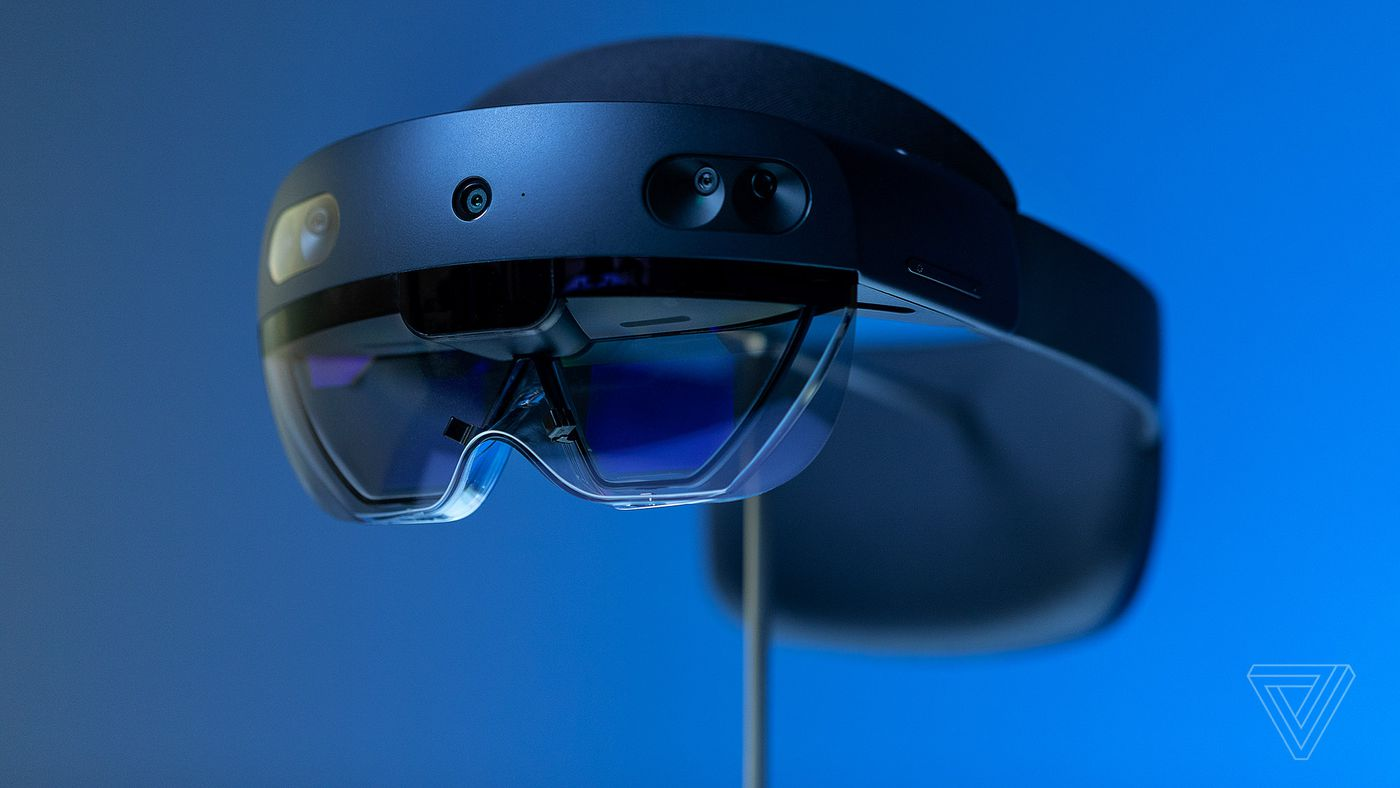
\includegraphics[width=130mm]{images/microsoft_hololens_2.jpg}
    \caption{Η συσκεύη μικτής πραγματικότητας Microsoft Hololens 2 {\footnotesize (Πηγή: theverge.com)}}\label{fig:hololensDevice}
\end{figure}

\subsection{Τεχνικά Χαρακτηριστικά}\label{subsec:hololensSpecs}
Η συσκεύη Microsoft Hololens 2, όπως και ο προκάτοχός του, αποτελεί ένα 'ασύρματο' ολογραφικό υπολογιστικό σύστημα. Το λειτουργικό του σύστημα είναι το Windows Holographic OS, το οποίο βασίζεται στo λειτουργικό σύστημα Windows 10~\cite{scooley_2023_hololens}. Ωστόσο, από το πρώτο εξάμηνο του 2023, η Microsoft δίνει τη δυνατότητα στους χρήστες της συσκεύης να την αναβαθμίσουν στο λειτουργικό σύστημα Windows 11~\cite{seiler_2023_microsoft}. Το headset αποτελείται από πολλά τμήματα/έξαρτηματα και αισθητήρες , όπως μπορούμε να παρατηρήσουμε με και στο \hyperref[fig:hololensDeviceParts]{\schema~\ref*{fig:hololensDeviceParts}}
\begin{figure}[!h]
    \centering
    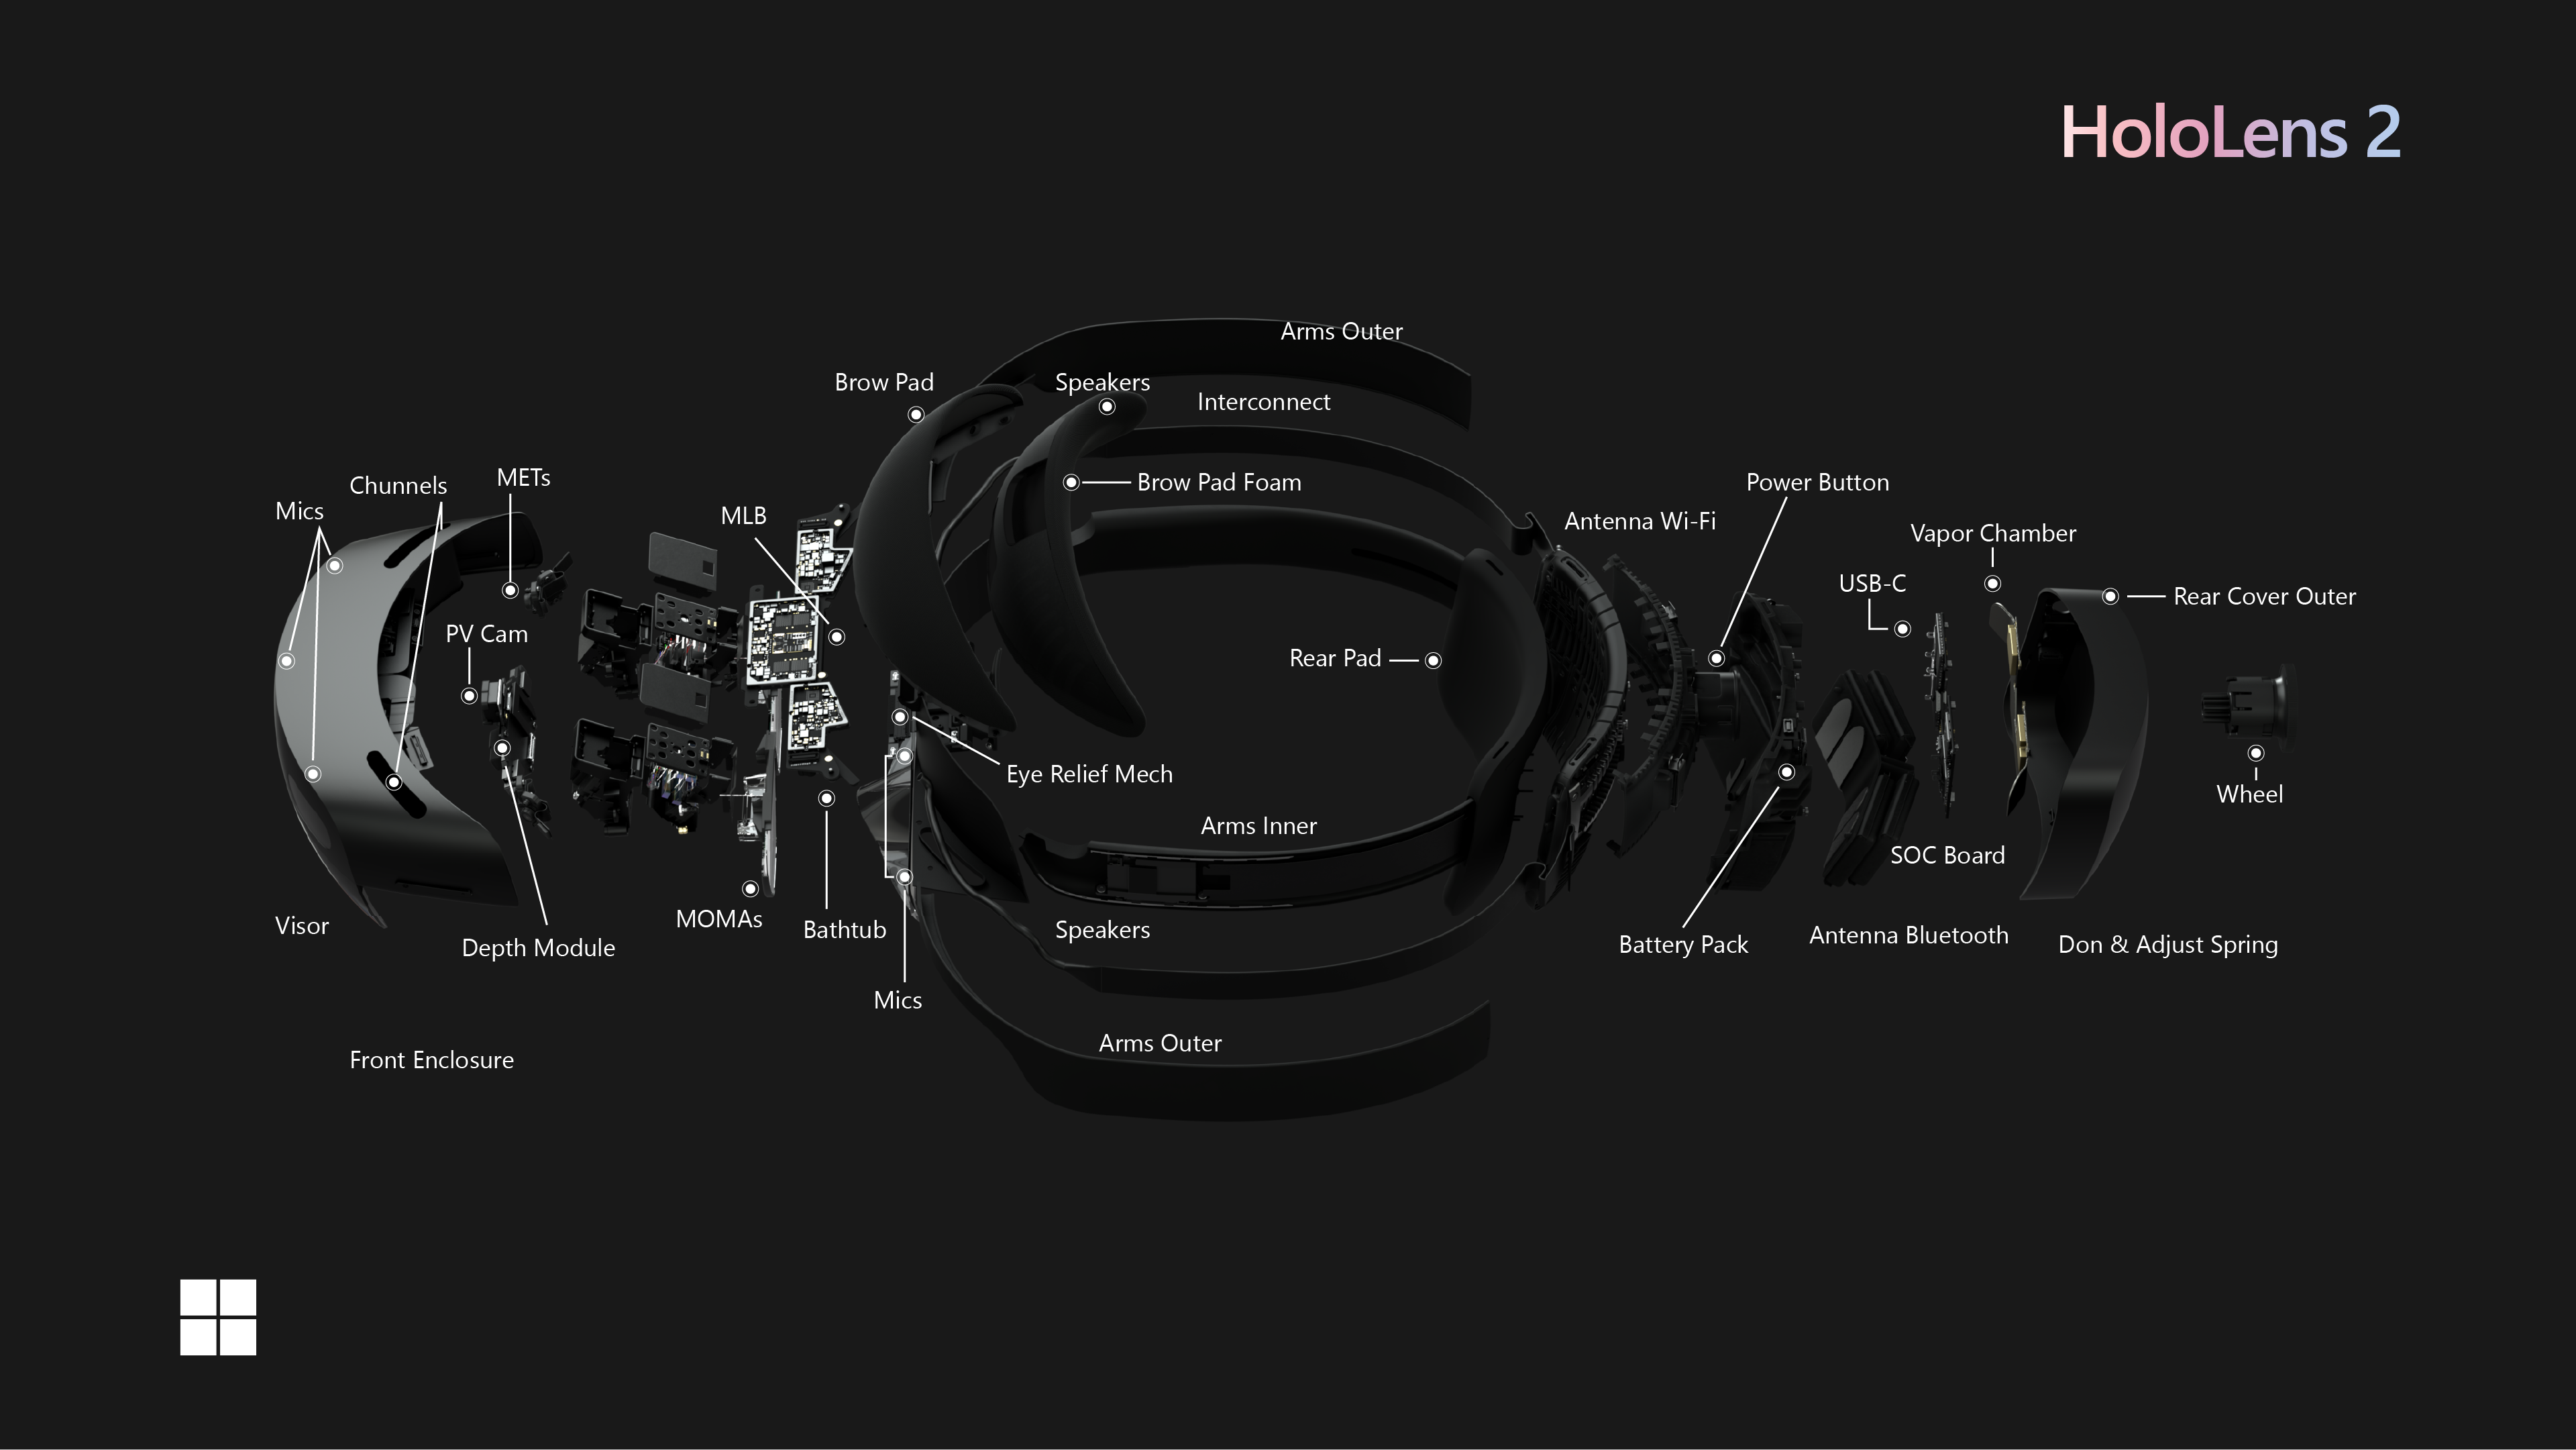
\includegraphics[width=130mm]{images/microsoft_hololens_2_parts2.png}
    \caption{Εξαρτήματα και αισθητήρες της συσκεύης Microsoft Hololens 2 {\footnotesize (Πηγή: learn.microsoft.com)}}\label{fig:hololensDeviceParts}
\end{figure}

Αρχικά, τα εξαρτήματα από τα οποία αποτελείται η συσκευή είναι τα κατώθι~\cite{scooley_2023_hololens}\cite{microsoft_hololens}:
\begin{itemize}
    \item \textbf{Visor} (Προσωπίδα): Η προσωπίδα διαθέτει τους αισθητήρες και τις οθόνες. Επιπλέον, μπορεί να περιστραφεί προς τα πάνω κατά της χρήση της συσκεύης, σε περίπτωση που ο χρήστης δεν χρησιμοποιεί τις οθόνες και θέλει να παρατηρήσει κάτι στον πραγματικό περιβάλλοντα χώρο.
    \item \textbf{Headband} (Ζώνη κεφαλής): Η ζώνη περοβάλλει το κεφάλι του χρήστη και εξασφαλίζει τη σωστή και σταθερή τοποθέτησή της. Με χρήση μιας ροδέλας, στο πίσω μέρος της συσκευής, ο χρήστης μπορεί να ρυθμίσει πόσο `σφιχτή' ή `χαλαρή' είναι η ζώνη, κατά την αρεσκεία του.
    \item \textbf{Brightness Buttons} (Κουμπιά φωτεινότητας): Με τα κουμπιά ρύθμισης φωτεινότητας, τα όποια βρίσκονται στην αριστερή πλευρά της προσωπίδας, ο χρήστης μπορεί να προσαρμόσει την φωτεινότητα των οθονών ανάλογα με το φως του περιβάλλοντα χώρου.
    \item \textbf{Volume Buttons} (Κουμπιά ήχου): Τα κούμπια ρύθμισης της έντασης του ήχου βρίσκονται στη δεξιά πλευρά της προσωπίδας.
    \item \textbf{Power Button} (Κουμπί ενεργοποίησης): Το κουμπί ενεργοποίησης (και απενεργοποίησης) της συσκευής βρίσκεται στο δεξί μέρος του εξωτερικού καλύμματος στην πίσω πλευρά της συσκευής.
    \item \textbf{USB-C Port} (Θύρα τύπου USB-C): Η θύρα USB-C, η οποία βρίσκεται κάτω από το κουμπί ενεργοποίησης, χρησιμοποιείται για την φόρτιση της συσκευής και για τη σύνδεση αυτής με άλλες συσκευές.
\end{itemize}

Επιπλέον, η συσκευή διαθέτει ένα πλήθος από αισθητήρες, οι οποίοι, όπως αναφέρθηκε, βρίσκονται στο visor (\hyperref[fig:hololensDeviceVisor]{\schema~\ref*{fig:hololensDeviceVisor}}). Ειδικότερα, διαθέτει~\cite{scooley_2023_hololens}:
\begin{itemize}
    \item 4 κάμερες ορατού φωτός, κάθε μία από τις όποιες έχει πεδίο ορατότητας (Field of View, FOV) 96.1\textdegree. Οι κάμερες αυτές χρησιμοποιούνται για τον εντοπισμό της θέσης και του προσανατολισμού του κεφαλιού (\textbf{Head Tracking}).
    \item 2 κάμερες υπέρυθρου φωτός, οι οποίες χρησιμοποιούνται για τον εντοπισμό της κίνησης των ματιών και του βλέμματος (\textbf{Eye Tracking}).
    \item 1 Time-of-Flight αισθητήρα βάθους (\textbf{Depth}) του 1 megapixels, δηλαδή ένα αισθτήρα που μετρά αποστάσεις βάσει του χρόνου που χρειάζονται τα φωτόνια, που εκπέμπει, να χτυπήσουν ένα στόχο και να επιστρέψουν στο δέκτη του αισθητήρα. Σε συνδυασμό με τις  κάμερες υπέρυθρου φωτός, είναι εφικτή η χωρική χαρτογράφηση (\hyperref[subsec:hololensSpatialMapping]{Κεφάλαιο~\ref*{subsec:hololensSpatialMapping}}) του περιβάλλοντος χώρου. 
    \item 1 μονάδα μέτρησης αδράνειας (\textbf{Inertia Measurement Unit, IMU}), η οποία περιλαμβάνει επιταχυνσιόμετρο, γυροσκόπιο και μαγνητόμετρο.
    \item 1 κάμερα των 8 megapixels, η οποία καταγράφει και βίντεο σε ανάλυση 1080p και 30 FPS.
\end{itemize}
\begin{figure}[!h]
    \centering
    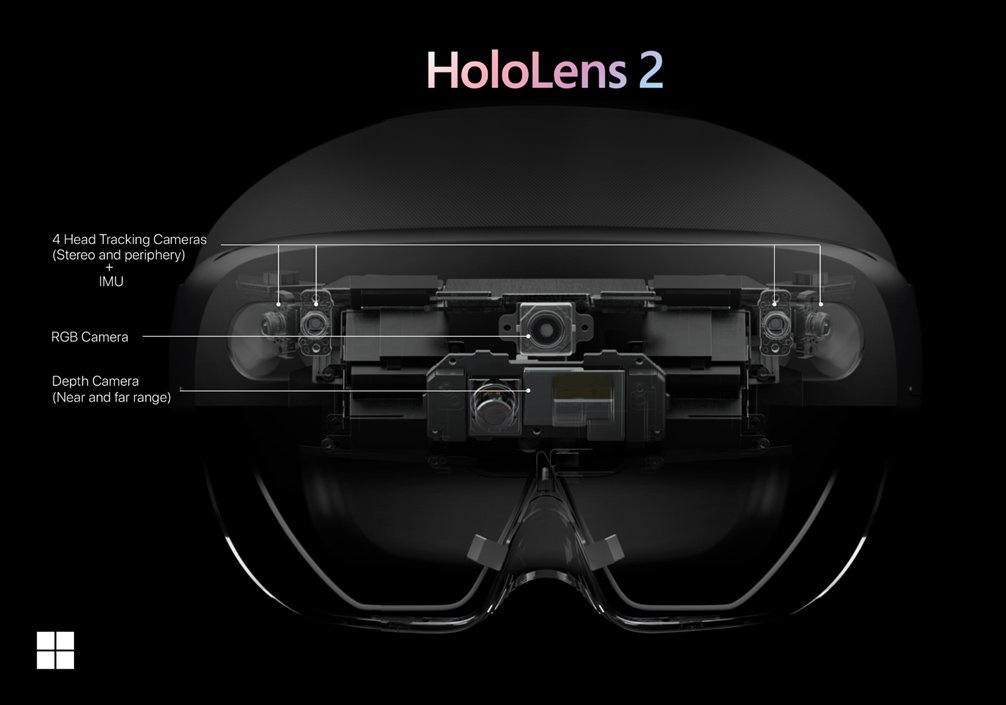
\includegraphics[width=100mm]{images/microsoft_hololens_2_parts1.png}
    \caption{Αισθητήρες στη προσωπίδα (visor) της συσκεύης Microsoft Hololens 2 {\footnotesize (Πηγή: learn.microsoft.com)}}\label{fig:hololensDeviceVisor}
\end{figure}

Τέλος, μερικές ακόμη σημαντικές προδιαγραφές της συσκευής αναφέρονται στον \hyperref[table:hololensSpecs]{Πίνακα~\ref*{table:hololensSpecs}}.
\begin{table}[!h]
    \begin{tabularx}{\textwidth}{|X|X|}
        \hline
        \textbf{Μικρόφωνο} & Συστοιχία 5 καναλιών \\
        \hline
        \textbf{Ηχείο} & Ενσωματώνει τεχνολογία χωρικού ήχου (\hyperref[subsec:hololensSpatialAudio]{Κεφάλαιο~\ref*{subsec:hololensSpatialAudio}}) \\
        \hline
        \textbf{System-on-Chip} & Qualcomm Snapdragon 850 Compute Platform \\
        \hline
        \textbf{Holographic Processing Unit} (Ολογραφική Μονάδα Επεξεργασίας) & Δεύτερης γενιάς, ειδικά κατασκευασμένη Holographic Processing Unit \\
        \hline
        \textbf{Μνήμη} & 4GB \\
        \hline
        \textbf{Αποθηκευτικός Χώρος} & 64GB \\
        \hline
        \textbf{WiFi} & 802.11ac 2x2 \\%chktex 29
        \hline
        \textbf{Bluetooth} & 5.0 \\
        \hline
        \textbf{Βάρος} & 566 γραμμάρια \\
        \hline
    \end{tabularx}
    \caption{Τεχνικές προδιαγραφές του headset Microsoft Hololens 2}\label{table:hololensSpecs}
\end{table}

\subsection{Τρόποι Αλληλεπίδρασης}\label{subsec:hololensInteraction}
Ο χρήστης έχει στη διάθεση τρεις βασικούς τρόπους με τους οποίους μπορεί να αλληλεπιδράσει με τη συσκευή και τα ολογράμματα που δημιουργεί~\cite{scooley_2023_hololens}:
\begin{enumerate}
    \item \textbf{Με εντοπισμό και χρήση των χεριών (Hand Tracking)}: Είναι δυνατός ο εντοπισμός των κινήσεων και των δύο χεριών, καθώς και των δαχτύλων αυτών, όταν αυτά βρίσκονται εντός του πεδίου ορατότητας (FOV) της συσκευής. Τα εικονικά χέρια που δημιουργούνται για την αλληλεπίδραση αποτελούν ένα σύνολο σημείων (\hyperref[fig:handRepresentation]{\schema~\ref*{fig:handRepresentation}}), όπου κάθε ένα αντιπροσωπεύει σύνδεσμο των χεριών ή σημεία αυτών~\cite{keveleigh_2022_hand}.
    
    \begin{figure}[!hb]
        \centering
        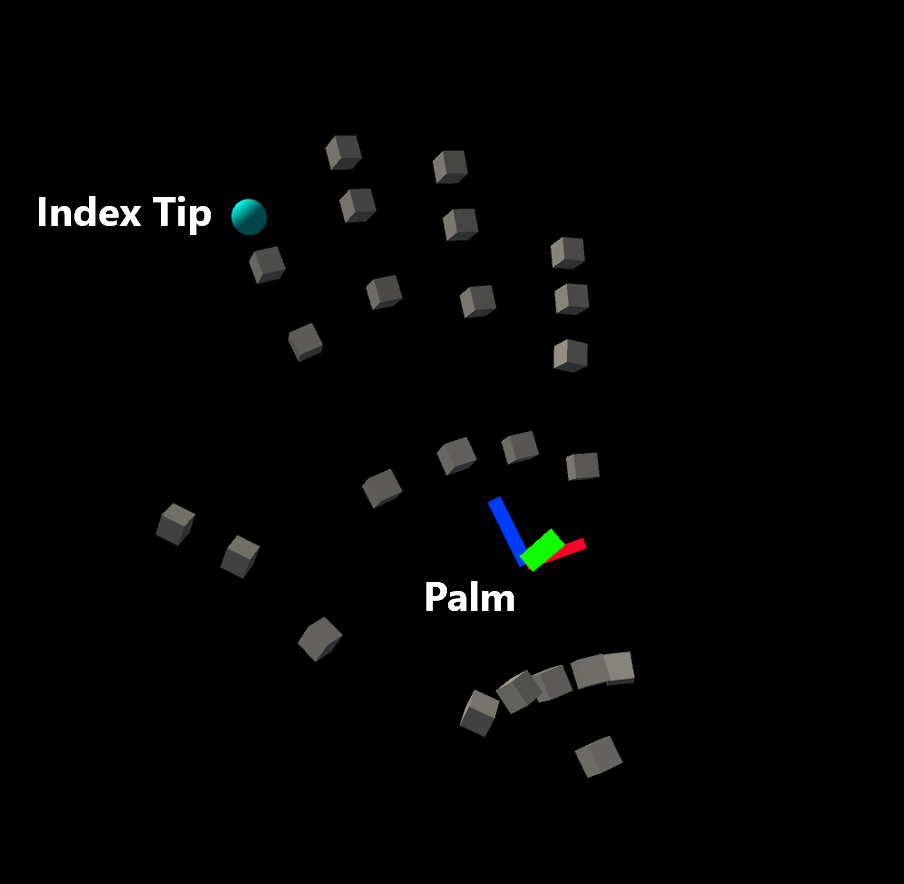
\includegraphics[width=0.5\textwidth]{images/holographic_hand.png}
        \caption{Εικονική αναπαράσταση χεριού {\footnotesize (Πηγή: learn.microsoft.com)}}\label{fig:handRepresentation}
    \end{figure}
    
    Ο χρήστης μπορεί να αληλεπιδράσει με τα εικονικά αντικείμενα, είτε από κοντινή~\cite{caseymeekhof_2022_direct}, είτε από μακρινή απόσταση~\cite{caseymeekhof_2022_point} και να πραγματοποιήσει συγκεκριμένες χειρονομίες (Gestures), όπως είναι το Air Tap, το Tap and Hold~\cite{sostel_2023_gaze} και το Start Gesture (επιτρέπει την πρόσβαση στο κεντρικό μενού)~\cite{shengkait_2022_start}, ώστε να υποδείξει την ενέργεια που επιθυμεί. Για παράδειγμα, με τους δείκτες των χέριων, ο χρήστης μπορεί να αγγίξει αντικείμενα (Touch) (\hyperref[fig:hololensInteractionTouch]{\schema~\ref*{fig:hololensInteractionTouch}}), να πιέσει κουμπιά (Press) (\hyperref[fig:hololensInteractionPress]{\schema~\ref*{fig:hololensInteractionPress}}), να κάνει ανακύλιση μιας σελίδας (Scroll) (\hyperref[fig:hololensInteractionScroll]{\schema~\ref*{fig:hololensInteractionScroll}}) ή να κάνει Zoom (\hyperref[fig:hololensInteractionZoom]{\schema~\ref*{fig:hololensInteractionZoom}})~\cite{caseymeekhof_2022_direct}.
    
    \begin{figure}[t]
        \centering
        \begin{subfigure}{0.3\textwidth}
            \centering
            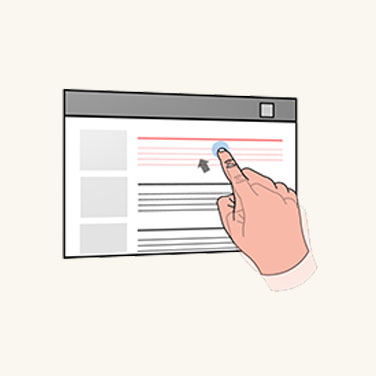
\includegraphics[width=0.9\linewidth]{images/hololens_interaction_touch.jpg}
            \caption{Touch}\label{fig:hololensInteractionTouch}
        \end{subfigure}%
        \begin{subfigure}{0.3\textwidth}
            \centering
            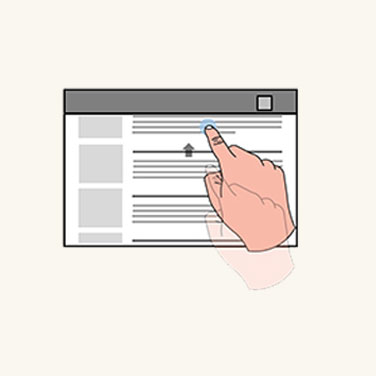
\includegraphics[width=0.9\linewidth]{images/hololens_interaction_scroll.jpg}
            \caption{Scroll}\label{fig:hololensInteractionScroll}
        \end{subfigure}%
        \begin{subfigure}{0.3\textwidth}
            \centering
            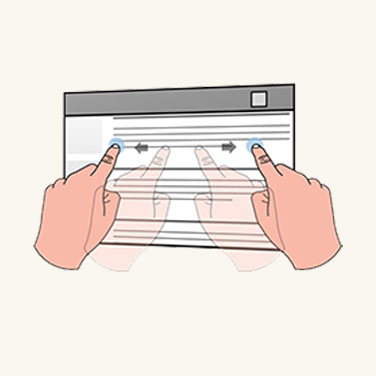
\includegraphics[width=0.9\linewidth]{images/hololens_interaction_zoom.jpg}
            \caption{Zoom}\label{fig:hololensInteractionZoom}
        \end{subfigure}%
        \caption{Τρόποι αλληλεπίδρασης με τους δείκτες των χεριών με 2D αντικείμενα {\footnotesize (Πηγή: learn.microsoft.com)}}\label{fig:hololensInteraction2D}
    \end{figure}
    \begin{figure}[!ht]
        \centering
        \begin{subfigure}{0.25\textwidth}
            \centering
            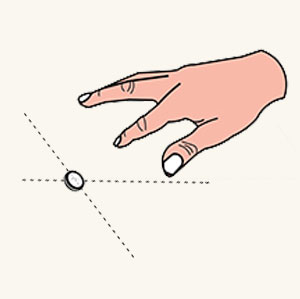
\includegraphics[width=0.9\linewidth]{images/hololens_interaction_press_step1.jpg}
        \end{subfigure}%
        \begin{subfigure}{0.25\textwidth}
            \centering
            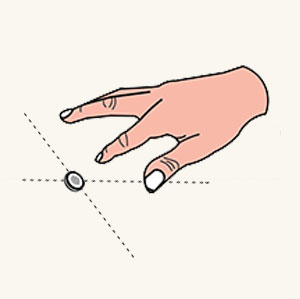
\includegraphics[width=0.9\linewidth]{images/hololens_interaction_press_step2.jpg}
        \end{subfigure}%
        \begin{subfigure}{0.25\textwidth}
            \centering
            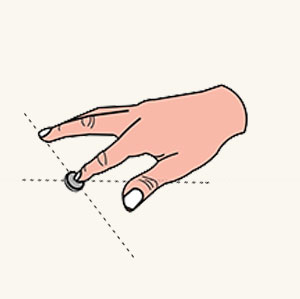
\includegraphics[width=0.9\linewidth]{images/hololens_interaction_press_step3.jpg}
        \end{subfigure}%
        \begin{subfigure}{0.25\textwidth}
            \centering
            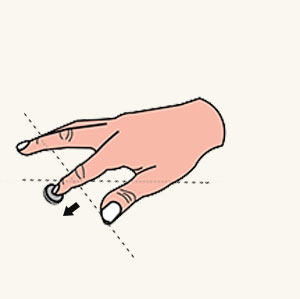
\includegraphics[width=0.9\linewidth]{images/hololens_interaction_press_step4.jpg}
        \end{subfigure}%
        \caption{Πίεση (Press) εικονικού κουμπιού {\footnotesize (Πηγή: learn.microsoft.com)}}\label{fig:hololensInteractionPress}
    \end{figure}

    \begin{figure}[!ht]
        \centering
        \begin{subfigure}{0.3\textwidth}
            \centering
            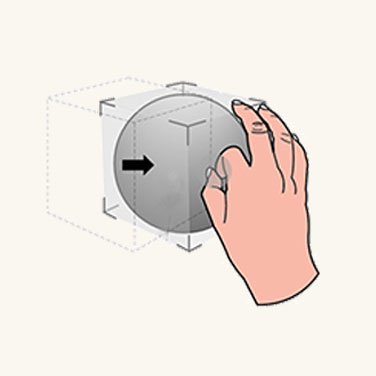
\includegraphics[width=0.9\linewidth]{images/hololens_interaction_move.jpg}
            \caption{Move}\label{fig:hololensInteractionMove}
        \end{subfigure}%
        \begin{subfigure}{0.3\textwidth}
            \centering
            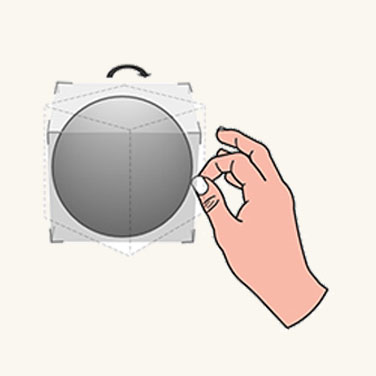
\includegraphics[width=0.9\linewidth]{images/hololens_interaction_rotate.jpg}
            \caption{Rotate}\label{fig:hololensInteractionRotate}
        \end{subfigure}%
        \begin{subfigure}{0.3\textwidth}
            \centering
            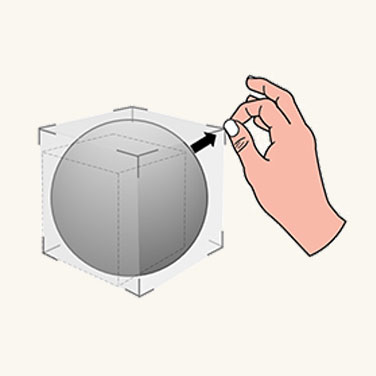
\includegraphics[width=0.9\linewidth]{images/hololens_interaction_scale.jpg}
            \caption{Scale}\label{fig:hololensInteractionScale}
        \end{subfigure}%
        \caption{Τρόποι αλληλεπίδρασης με το δείκτη και τον αντίχειρα με 3D αντικείμενα {\footnotesize (Πηγή: learn.microsoft.com)}}\label{fig:hololensInteraction3D}
    \end{figure}
    
    Αν ο χρήστης κρατήσει τον αντίχειρα και τον δείκτη ενωμένο, τότε μπορεί να μετακινήσει (Move) (\hyperref[fig:hololensInteractionMove]{\schema~\ref*{fig:hololensInteractionMove}}) και να αλλάξει την κλίμακα (Scale) (\hyperref[fig:hololensInteractionScale]{\schema~\ref*{fig:hololensInteractionScale}}), τόσο δισδιάστατων (2D), όσο και τρισδιάστατων (3D) αντικειμένων. Επιπλέον, για τα 3D εικονικά αντικείμενα, με την ίδια χειρονομία (gesture), μπορεί να τα περιστρέψει (Rotate) (\hyperref[fig:hololensInteractionRotate]{\schema~\ref*{fig:hololensInteractionRotate}}). Το σημείο επαφής με το αντικείμενο είναι αυτό το οποίο καθορίζει ποια ένεργεια από τις τρεις ανωτέρω θα πραγματοποιήσει ο χρήστης~\cite{caseymeekhof_2022_direct}.
    
    Τέλος, οι ίδιες ενέργειες που αναφέρθηκαν ως τώρα, μπορούν να πραγματοποιηθούν και σε εικονικά αντικείμενα που βρίσκονται μακριά από το χρήστη (σε απόσταση μεγαλύτερη των 50 εκατοστών). Από το δάκτυλο του χρήστη εκτείνεται μια ακτίνα, στο τέλος του οποίου υπάρχει ένας κέρσορας, ώστε να διευκολύνει τον χρήστη να αντιληφθεί ποιο είναι το σημείο αλληλεπίδρασης με το αντικείμενο~\cite{caseymeekhof_2022_point}. Ο ίδιος δείκτης εμφανίζεται και κατά την αλληλεπίδραση με αντικείμενα σε κοντινή απόσταση.
    
    \begin{figure}[!h]
        \centering
        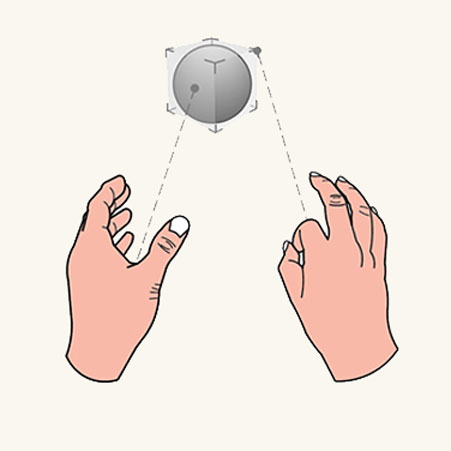
\includegraphics[width=0.5\linewidth]{images/hololens_interaction_far_manipulation.jpg}
        \caption{Αλληλεπίδραση με εικονικό αντικείμενο σε μακρινή απόσταση {\footnotesize (Πηγή: learn.microsoft.com)}}
    \end{figure}

    \item \textbf{Με το βλέμα και την κίνηση των ματιών ή του κεφαλιού (Gaze and Dwell)}~\cite{sostel_2022_gaze}: Ο χρήστης ελέγχει ένα κέρσορα, τον οποίο μπορεί να μετακινήσει εντός του FOV, χρησιμοποιόντας είτε την κίνηση του κεφαλιού του~\cite{seankerawala_2022_headgaze}, είτε την κίνηση των ματιών (Eye Tracking)~\cite{sostel_2023_eyegaze}. Αυτός ο τρόπος αλληλεπίδρασης μπορεί να αποδειχθεί ιδιαίτερα χρήσιμος, σε περίπτωση που ο χρήστης αδυνατεί να χρησιμοποιήσει τα χέρια του, επειδή, για παράδειγμα, κρατά κάποιο εργαλείο ή αντιμετωπίζει κάποια δυσκολία ή πρόβλημα υγείας, ενώ έχει ακόμη μεγαλύτερη χρηστικότητα, αν συνδυαστεί με φωνητικές εντολές~\cite{sostel_2023_gaze}\cite{hak0n_2022_voice}.
    \item \textbf{Με φωνητικές εντολές (Voice Input)}: Ο χρήστης έχει την δυνατότητα να χρησιμοποιήσει φωνητικές εντολές, ώστε να επιτελέσει ενέργειες. Η συσκευή ακολουθεί το μοντέλο `See It, Say It', οπότε οι εντολές που μπορούν να χρησιμοποιηθούν υποδεικνύονται με ετικέτες (\hyperref[fig:hololensInteractionVoice]{\schema~\ref*{fig:hololensInteractionVoice}}) και κουμπιά. Τέλος, αυτός ο τρόπος αλληλεπίδρασης μπορεί να συνδυάστει με οποιονδήποτε από τους δύο προηγούμενους για λόγους ευκολίας ή/και αύξησης απόδοσης~\cite{hak0n_2022_voice}.
    
    \begin{figure}[!h]
        \centering
        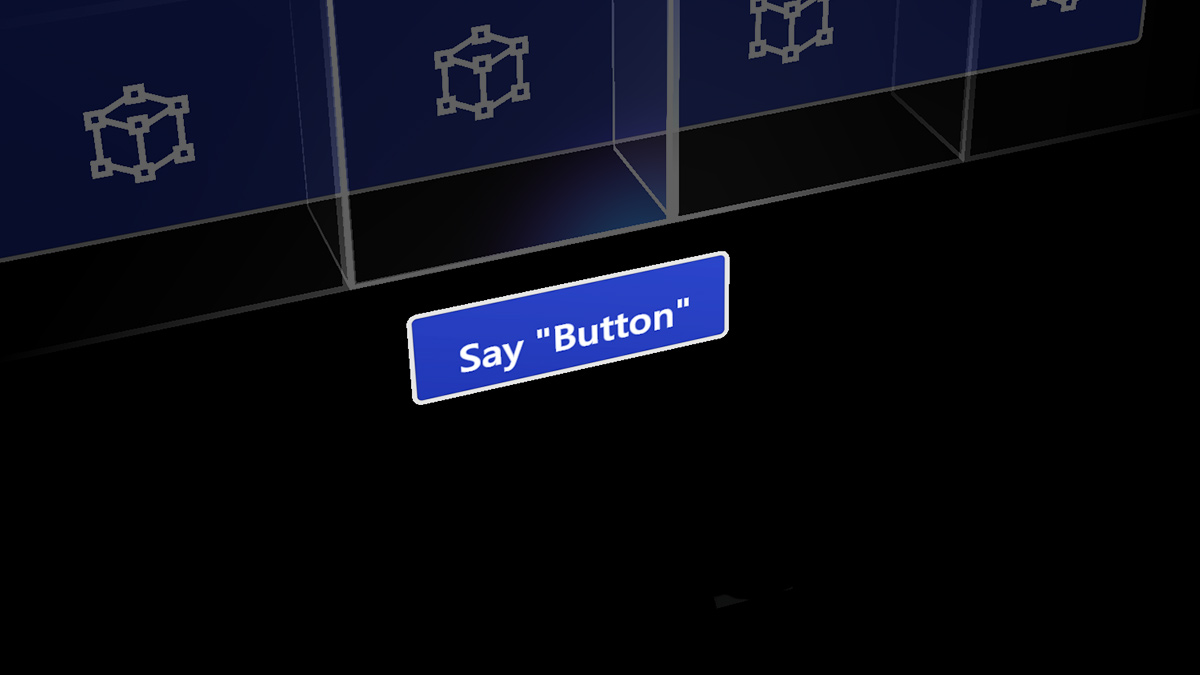
\includegraphics[width=0.8\textwidth]{images/hololens_interaction_voice.jpg}
        \caption{Ετικέτα υποδεικνύει την φωνητική εντολή {\footnotesize (Πηγή: learn.microsoft.com)}}\label{fig:hololensInteractionVoice}
    \end{figure}
\end{enumerate}

\subsection{Χωρική Χαρτογράφηση (Spatial Mapping)}\label{subsec:hololensSpatialMapping}
Η χωρική χαρτογράφηση (spatial mapping) αποτελεί μία από τις κύριες δυνατότητες της συσκεύης Microsoft Hololens και είναι το κύριο χαρακτηριστικό, στο οποίο στηρίζονται οι εφαρμογές που αναπτύσσονται για τη συσκευή για να υλοποιήσουν τις λειτουργίες μικτής πραγματικότητας. Χωρική χαρτογράφηση είναι η σάρωση και η δημιουργία μίας 3D αναπαράστασης του περιβάλλοντος χώρου του χρήστη (\hyperref[fig:spatialMappingExample]{\schema~\ref*{fig:spatialMappingExample}}). Αυτό επιτρέπει στα εικονικά αντικείμενα να αλληλεπιδρούν με αντικείμενα του πραγματικού χώρου, κάθως στην πραγματικότητα αλληλεπιδρούν με το `πλέγμα' (mesh), το οποίο είναι ένα σύνολο κορυφών και πολυγώνων (συνήθως τριγώνων) που αντιπροσωπεύουν το αντικείμενο~\cite{a2006_mesh}, δρώντας ως το εικονικό του αντίγραφο, προσδίδοντας στο χρήστη την ψευδαίσθηση ότι τα αντικείμενα βρίσκονται όντως στο περιβάλλοντα χώρο~\cite{mattzmsft_2023_spatial}.

\begin{figure}[!h]
    \centering
    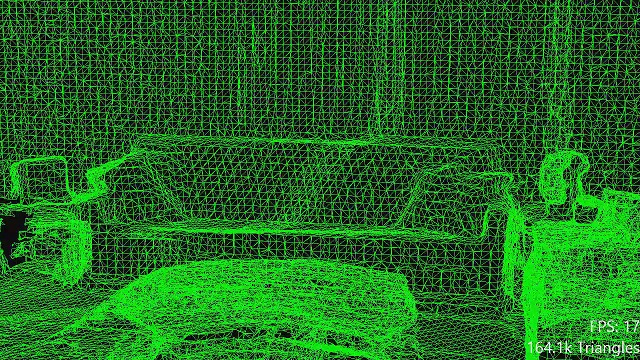
\includegraphics[width=0.8\textwidth]{images/spatial_mapping_example.jpg}
    \caption{Τριασδιάστατη ανάπαρασταση ένος χώρου {\footnotesize (Πηγή: learn.microsoft.com)}}\label{fig:spatialMappingExample}
\end{figure}

Σε αντίθεση με το Hololens 1, το Hololens 2 μπορεί να αξιοποιήσει τα δεδομένα που λαμβάνονται από το spatial mapping και, σε συνδυασμό με τεχνητή νοημοσυνή, να σχηματίζει περιοχές (Quads), ομαδοποιόντας πολύγωνα που μπορεί να ανήκουν στο ίδιο πραγματικό αντικείμενο ή/και επιφάνεια (π.χ. τοίχος, πάτωμα, τραπέζι κ.λ.π.) (\hyperref[fig:sceneUnderstandingExample]{\schema~\ref*{fig:sceneUnderstandingExample}}). Με αυτό τον τρόπο, τα δεδομένα αποκτούν μια δομή, καθιστώντας τα πιο κατανοητά στον προγραμματιστή, που επιθυμεί να τα χρησιμοποιήσει~\cite{szymons_2022_scene}. Αυτό επιτυγχάνεται με το Scene Understanding SDK, το οποίο, πέρα των πλεονεκτημάτων που περιγράφηκαν προηγουμένων, φέρει και ορισμένα μειονεκτήματα σε σχέση με το spatial mapping, όπως είναι η καθυτσέρηση ανανέωσης των δεδομένων, καθώς τα δέδομενα που αξιοποιεί είναι στατικά~\cite{mattzmsft_2023_spatial}.

Οι κυριότεροι λόγοι χρήσης της τεχνολογίας της χωρικής χαρτογράφησης είναι~\cite{mattzmsft_2023_spatial}:
\begin{itemize}
    \item Η τοποθέτηση εικονικών αντικειμένων σε πραγματικές επιφάνειες.
    \item Η απόκρυψη εικονικών αντικειμένων, όταν βρίσκονται πίσω από πραγματικές επιφάνειες.
    \item Η εφαρμογή φυσικής σε εικονιικά αντικείμενα. Με αυτό τον τρόπο, τα ολογράμματα μπορούν να αλληλεπιδρούν με πιο ρεαλιστικό τρόπο με τα πραγματικά αντικείμενα.
    \item Η πλοήγηση εικονικών αντικειμένων, καθώς και χρηστών, στον πραγματικό χώρο.
\end{itemize}

Τέλος, πρέπει να υπογραμμιστεί ότι υπάρχει ένας αριθμός παραγόντων, οι οποίοι μπορεί να επηρέασουν την αποτελεσματικότητα και την ακρίβεια της χωρικής χαρτογράφησης. Τέτοιο παράγοντες είναι ο φωτισμός του χώρου, η έλλειψη ύπαρξης αναγνωρίσημων χαρακτηριστικών πάνω σε απλές επιφάνειες, η ύπαρξη wormholes (σημεία του χώρου που φέρουν τα ίδια ή παρόμοια χαρακτηριστικά, με αποτέλεσμα, να θεωρούνται, εσφαλμένα, από τη συσκευή ως ο ίδιος χώρος), οι συχνές αλλαγές και κινήσεις στο χώρο, οι ανακλαστικές επιφάνειες κ.α.~\cite{dorreneb_2022_hololens}.

\begin{figure}[!h]
    \centering
    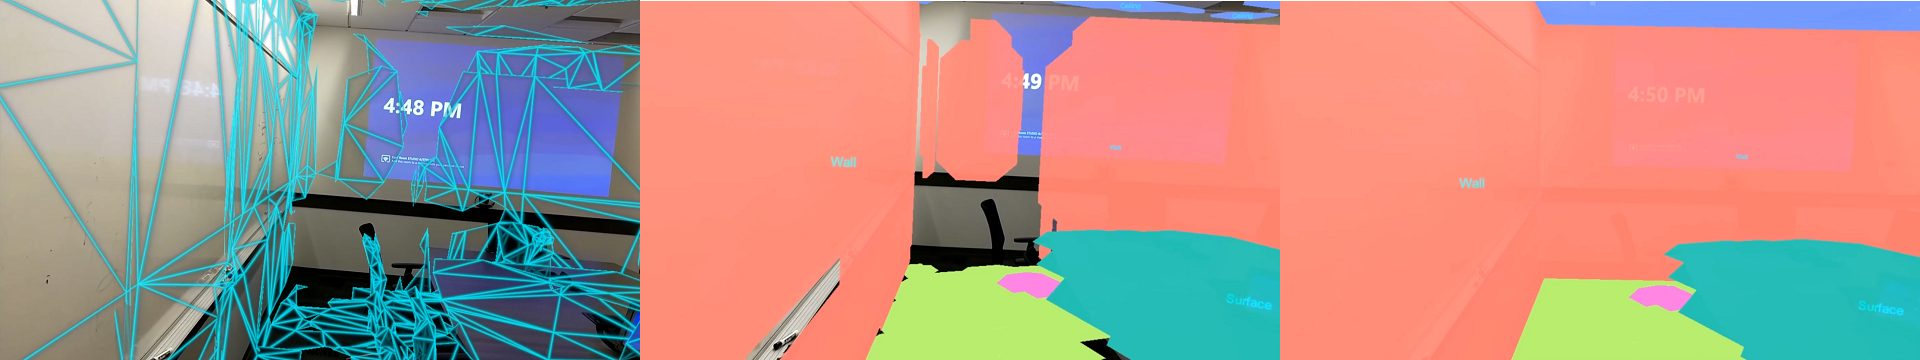
\includegraphics[width=1\textwidth]{images/sm_and_su_comparisson.png}
    \caption{Περιοχές (Quads) που σχηματίστηκαν από το Scene Understanding {\footnotesize (Πηγή: learn.microsoft.com)}}\label{fig:sceneUnderstandingExample}
\end{figure}

\subsection{Χωρικός Ήχος (Spatial Audio)}\label{subsec:hololensSpatialAudio}
Η συσκευή Microsoft Hololens 2 ενσωματώνει, επίσης, την τεχνολογία χωρικού ήχου, η οποία συνεισφέρει ακόμη περισσότερο στη μίξη του πραγματικού και του εικονικού κόσμου, προσφέροντας μια ρεαλιστική εμπειρία στο χρήστη. Η τεχνολογία βασίζεται στην ικανότητα του ανθρώπου να αντιληφθεί την θέση και την κατεύθυνση από την οποία προήλθε κάποιος ήχος. Με τη χρήση των δύο ηχείων, τα οποία βρίσκονται εκατέρωθεν του κεφαλιού του χρήστη, και τεχνολογίας βασισμένη στη Head-related συνάρτηση μεταφοράς (Head-related Transfer Function, HRTF), είναι εφικτό η συσκευή να παράγει ήχο, για τον όποιο, θα είναι εφικτό ο χρήστης να υποδείξει την κατεύθυνση προέλευσης αυτού~\cite{kegodin_2022_spatial}. Η HRTF αποτελεί το λόγο του μετασχηματισμού Fourier της πίεσης του ήχου στην είσοδου του καναλιού του αυτιού και της πίεσης αυτής στο μέσο του κεφαλιού~\cite{henrikmller_1992_fundamentals}. Ανάλογα με το σχήμα και το μέγεθος του αυτιού του χρήστη, η συσκευή μπορεί να προσαρμόσει την HRTF με σκοπό να βελτιώσει την εμπειρία του χρήστη. Το spatial audio χρησιμοποιείται κυρίως για να τραβήξουμε την προσοχή του χρήστη προς κάποια συγκεκριμένη κατεύθυνση ή κάποιο συγκεκριμένο ολόγραμμα, το οποίο μπορεί να βρίσκεται εκτός του πεδίου ορατότητάς του~\cite{kegodin_2022_spatial}.